\documentclass[25pt, a0papper, portrait]{tikzposter}
\usepackage[utf8]{inputenc}
 
\title{Extracting Semantic Frames using Handwritten \texttt{hfst-pmatch Rules}}
\author{Sam Hardwick, Miikka Silfverberg and Krister Lind{é}n}
\date{\today}
\institute{University of Helsinki}
 
\usepackage{amsmath}
\usepackage{xyling}
\usepackage{graphicx}
 
\usetheme{Desert}
 
\begin{document}
 
\maketitle
 
 
\begin{columns}
    \column{0.5}
    \block{A Semantic Frame}{
      A semantic frame is a description of a \emph{type} of event, relation or entity
      and related participants.
      \vspace{2cm}
      $$
  \Big[_\text{Size}\Big[_\text{Entity}\text{He} \Big]
  \text{is} \Big[_\text{Degree} \text{quite} \Big] \Big[_\text{Lexical Unit}\text{tall} \Big]
  \Big[_\text{Standard} \text{for a jockey} \Big] \Big]
  $$

  \vspace {2cm}

  Tagging it and its parts is \emph{frame extraction}.
\vspace{1cm}

  We demonstrate an extraction approach to one particular frame, \emph{Size}. It
has the following elements:
\vspace{1cm}

\begin{center}
  \begin{tabular}{ l | l }
Lexical Unit (LU) & Adjective describing magnitude (large, tiny, ...) \\ \hline
Entity & That which is being described (house, debt, ...) \\ \hline
Degree, optional & Intensity or extent of description (really, quite, ...) \\ \hline
Standard, optional & A point of comparison (for a jockey, ...) \\
    \end{tabular}
\end{center}
      
%      A bracketed diagram and some text
    }
%\block{Context-}{foo}
    
    \column{0.5}
    \block{Surface Syntactic Representation}{

      We describe the frame and its elements with a form of surface syntax.

      \vspace{2cm}
\begin{center}
  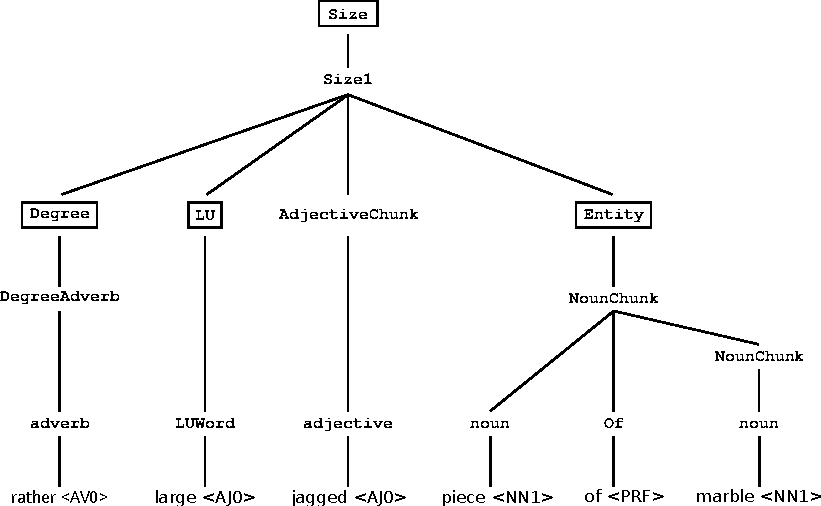
\includegraphics[width=32cm]{images/tagged_tree1.pdf}
  \end{center}
      
      %% \Tree[7]{
      %%   & & & \K{Size1} \B{dll} & & & \\
      %%   \K{Degree} \B{d} & & & & & & \\
      %%   \K{rather} & \K{large} jagged & \K{chunk} & \K{of} & \K{the} & \K{marble} & \K{statue}
      %% }

      \vspace{2cm}

      Our finite-state -based formalism permits context-free rules; here, \textbf{NounChunk} appears in its own production.


}
\end{columns}

 \block{Rule design and training}
 {
   Full-width block with big flowchart:
   
 }

 \begin{columns}
   \column{0.4}{
     \block{Formalism and implementation}{
     \texttt{hfst-pmatch} is a development of Xerox's \texttt{fst} and its command \texttt{pmatch}.
     It is a regular expression compiler that inserts tags around recognised parts of the input.

\vspace{0.6cm}
\begin{center}
{\Large \texttt{<Entity>ball and chain</Entity>}}
\end{center}

\vspace{0.6cm}

     It features fast left-to-right longest-match tagging, recursive transition network -style arcs (which allows context-free parsing) and runtime context-checking.

\vspace{1cm}
\begin{center}
 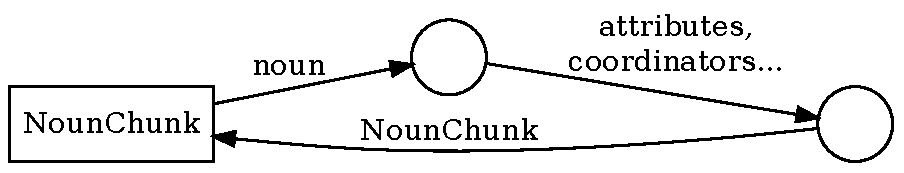
\includegraphics[width=22cm]{images/rtn.pdf}
\end{center}
     }
   }
   \column{0.6}{
     \block{Evaluation}{
       For a single frame such as \emph{Size}, proper evaluation is challenging due to lack of systematic reference corpora.
       We tagged 200 sentences for training and 100 for evaluation ourselves, with the following results:

\begin{center}
  \begin{tabular}{l | l}
    \hline
    Number of sentences & 100 \\
    Number of LUs & 113 \\
    Number of LUs corresponding to a \verb+Size+ frame & 56 \\ %non-sizes = 57
    Number thereof matched by the rules & 50 \\
    Total number of matches made by the rules & 54 \\
    \hline
    Coverage & 89\% \\
    Accuracy & 93\% \\
    \hline
  \end{tabular}
\end{center}
       }
}
   \end{columns}

 
%% \begin{columns}
%%     \column{0.8}
%%     \block{A figure}
%%     {
%%         %% \begin{tikzfigure}
%%         %%     
\includegraphics[width=0.4\textwidth]{images/logo.png}
%%         %% \end{tikzfigure}
%%     }
%%     \column{0.2}
%%     \block{Or maybe have description to right}{}
%% \end{columns}
 
\end{document}
